\documentclass[aspectratio=1610,12pt,xcolor=dvipsnames]{beamer}
\mode<presentation>

% Respect chosen fonts (serif) and metrics
\usefonttheme{professionalfonts}
\renewcommand{\familydefault}{\rmdefault}

% Figures
\usepackage{graphicx}
\usepackage{float}

%% table
\usepackage{xcolor}
\usepackage{fancyhdr}
\usepackage{booktabs}
\usepackage[table]{xcolor}

% subsection page template
\setbeamertemplate{subsection page}
{
  \begin{centering}
    \vfill
    {\usebeamerfont{section title}\usebeamercolor[fg]{section title}\Large\insertsubsectionhead\par}
    \vfill
  \end{centering}
}
% section page template
\setbeamertemplate{section page}
{
  \begin{centering}
    \vfill
    {\usebeamerfont{section title}\usebeamercolor[fg]{section title}\Large\insertsectionhead\par}
    \vfill
  \end{centering}
}

%% footnote
\setbeamertemplate{footnote}{%
  \parindent 0em\noindent%
  \raggedright\insertfootnotemark\insertfootnotetext\par%
}

%% theme
\usetheme{default}
\useoutertheme{miniframes}
\definecolor{nagivation}{rgb}{0,0,0.35} % (typo kept if intentional)
\definecolor{main}{rgb}{0,0,0.5}
\setbeamercolor{structure}{bg=white,fg=nagivation}
\setbeamercolor{frametitle}{fg=nagivation}
\setbeamercolor{section in head/foot}{fg=white,bg=nagivation}
\setbeamertemplate{footline}[page number]
\setbeamertemplate{items}[circle]
\setbeamerfont{footnote}{size=\footnotesize}
\setbeamerfont{caption}{size=\footnotesize}
\setbeamertemplate{subsection in head/foot}{}%
\setbeamertemplate{subsection in head/foot shaded}{}%

%% font
\usepackage{dsfont}
\usepackage{newpxtext}
\usepackage{newpxmath}
\usepackage{amsmath}

% Math & bib
\usepackage{amsmath,amsfonts,amssymb,bm}
\DeclareMathOperator*{\argmin}{arg\,min}
\newcommand{\indep}{\perp\!\!\!\, \perp}
\usepackage{natbib}
\bibliographystyle{asr}
\setcitestyle{aysep={}}
\usepackage[english]{babel}

\makeatletter
\DeclareRobustCommand\citep
{\begingroup\scriptsize\color{gray}\NAT@swatrue\let\NAT@ctype\z@\NAT@partrue
    \@ifstar{\NAT@fulltrue\NAT@citetp}{\NAT@fullfalse\NAT@citetp}}
\makeatother

% Roman numerals macro
\newcommand{\rom}[1]{\uppercase\expandafter{\romannumeral #1\relax}}

%% Title
\title[CML]{SOC 690S: Machine Learning in Causal Inference\\[1.5pt]}
\subtitle{\large Week 1: Motivation and Linear Regression\\[-10pt]}

%% author
\author[Jiang] 
{\large Wenhao Jiang\vspace{-2em}}

%% affiliation
\institute[Duke]{}
\titlegraphic{
\includegraphics[height=1.4cm]{Misc/duke_logo.png}}

\date[Duke]
{\large Department of Sociology, Fall 2025}

\begin{document}

%%%%%%%%%%%%%%%%%%%%%%%%%%%%%%%%%%%%
%%%%%%%%Begin Main Content%%%%%%%%%%
%%%%%%%%%%%%%%%%%%%%%%%%%%%%%%%%%%%%

%% Title page %%
\begin{frame}
    \titlepage 
\end{frame}

\section{Introduction}

\begin{frame}
  \sectionpage
\end{frame}

\begin{frame}{What to Expect in this Course}
\begin{itemize}
    \item This is an \textit{advanced statistics course} combining 
    \textit{causal inference} (statistical inference) 
    with \textit{prediction} (machine learning)
    \begin{itemize}
        \item Emphasis on both \textit{statistical theory} and \textit{sociological applications}
    \end{itemize} \pause
    \item This integration is a \textit{growing frontier}
    \begin{itemize}
        \item Driven by high-dimensional data ($p>n$)
        \item Enabled by flexible, non-linear models
    \end{itemize}
    \end{itemize}
\end{frame}

\begin{frame}{What to Expect in this Course}
\begin{itemize}
    \item This integration is a \textit{growing frontier} driven by high-dimensional data
    \begin{itemize}
        \item Driven by high-dimensional data ($p>n$)
        \item Wang et al. (2024) estimated the causal (hopeful) effect of biomarkers on Alzheimer’s Disease severity using high-dimensional genetic data
        \item Gupta and Lee (2023) decomposed causal effects of components in digital marketing interventions, where firms track thousands of features—such as user behavior, timestamps, and campaign attributes
    \end{itemize}
    \end{itemize}
\end{frame}

\begin{frame}{What to Expect in this Course}
\begin{itemize}
    \item This integration is a \textit{growing frontier} enabled by flexible, non-linear models
    \begin{itemize}
        \item Óskarsdóttir et al. (2020) incorporated mobile phone call-detail records and social network measures—vast, nontraditional datasets—into credit scoring models, using ML methods such as random forests and gradient boosting to flexibly estimate non-linear interactions among predictors
    \end{itemize}
    \end{itemize}
\end{frame}

\begin{frame}{Tips of Study}
\begin{itemize}
    \item I assume you have reasonable familiarity with \textit{Probability and Statistics}, and a basic understanding of \textit{Calculus} and \textit{Linear Algebra}
    \item However, you do not need to follow every step of the statistical derivations
    \item The focus is on developing \textit{intuition} (for example, how and why \textit{Double Machine Learning} works for statistical inference in high-dimensional data) and understanding how these methods may be applied in your research
    \begin{itemize}
        \item Homework and the midterm exam are intended as learning tools to strengthen your \textit{basic} statistics and build \textit{intuition}
    \end{itemize}
\end{itemize}
\end{frame}

\begin{frame}{Tips of Study}
\begin{itemize}
    \item I will go through the material at a deliberate pace
    \item The pace and content will remain flexible, tailored to your level and needs
    \item Don’t feel pressured if some statistical concepts are unclear at first
    \begin{itemize}
        \item Some topics are not immediately essential
        \item Others will become more familiar through repeated exposure
    \end{itemize}
    \item My slides are intentionally dense (to help me prepare), so please feel free to stop me at any point if something is unclear
\end{itemize}
\end{frame}

\subsection{Syllabus and Timeline}

\begin{frame}{}
\vspace{-1.4em}
\setlength{\tabcolsep}{1pt}
{\footnotesize\begin{table}[h!]
\centering
\begin{tabular}{@{}llp{9.8cm}cc@{}}
\hline \hline\\[-10pt]
\textbf{\textcolor{black}{Week}} & \textbf{\textcolor{black}{Date}} & \textbf{\textcolor{black}{Topic}} & \multicolumn{2}{c@{}}{\textbf{\textcolor{black}{Problem sets}}} \\
 & & & Assign & Due \\
\hline \\[-10pt]
1  & Aug 26  & Introduction: Motivation and Linear Regression &  &  \\
2  & Sep 2  & Foundation: Machine Learning Basics &  &  \\
3  & Sep 9  & Foundation: Machine Learning Advanced & 1 &  \\
4  & Sep 16  &  Foundation: Causal Inference Basics &  &  \\
5  & Sep 23  & Foundation: Causal Inference Advanced & 2 & 1 \\[4pt]
\arrayrulecolor{gray}
\hline \\[-9pt]
6  & Sep 30  & Core: PSM and Doubly Robust Estimation & & \\
8  & Oct 7    & Core: Instrumental Variable Estimation & 3 & 2  \\
7  & Oct 14  & \textit{Fall break} &  &  \\
9  & Oct 21  & \textbf{In-class midterm} &  & \\
10  & Oct 28  &  Core: Regression Discontinuity Design &  4 & 3 \\
11  & Nov 4  & Core: Panel Data and Difference-in-Difference & & \\[4pt]
\arrayrulecolor{gray}
\hline \\[-9pt]
12  & Nov 11    & Advanced: Heterogeneous Treatment Effect & 5 & 4 \\
13 & Nov 18    & Advanced: Unstructured Data Feature Engineering & & \\
14 & Nov 25   & Advanced: Causal Reasoning in Machine Learning &  & 5 \\
 & Dec 13   & \textbf{Take-home final} & & \\
\arrayrulecolor{black}
\hline \hline
\end{tabular}
\end{table}}
\end{frame}

%% FWL Theorem %%
\section{Linear Regression}

\subsection*{Linear Regression and Conditional Expectation Function (CEF)}

\begin{frame}
  \subsectionpage
\end{frame}

\begin{frame}{Conditional Expectation Function (CEF)}
    \begin{itemize}
        \item In a \textit{population}, given a dependent variable $Y_i$ and a $p \times 1$ vector of covariates $X_i$, the \textit{best predictor} of $Y_i$ given $X_i$ is
        \begin{align*}
            g(X_i) = E[Y_i \mid X_i]
        \end{align*}
        in the sense of minimizing mean squared error (MMSE)
        \item $X_i$ is a random variable, and $E[Y_i \mid X_i]$, as a function of $X_i$, is also a random variable
        \item We sometimes work with a particular value of CEF
        \begin{align*}
            E[Y_i \mid X_i = x] = \int tf_y(t \mid X_i = x)dt
        \end{align*}
    \end{itemize}
\end{frame}

\begin{frame}{Conditional Expectation Function (CEF)}
    \begin{itemize}
        \item Suppose $X_i$ is years of completed education, $Y_i$ is weekly earnings
        \begin{figure}
            \centering
            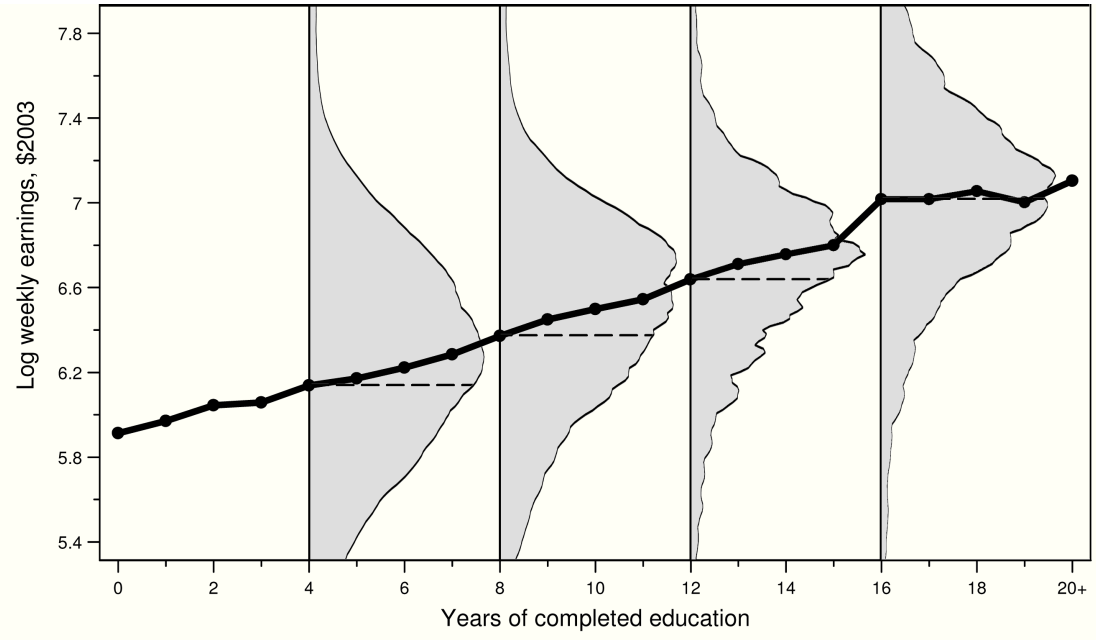
\includegraphics[width=0.7\linewidth]{Linear Regression/Figures/CEF_education.png}
            \caption{The CEF of average weekly earnings given schooling}
            \label{fig:CEF_education}
        \end{figure}
    \end{itemize}
\end{frame}

\begin{frame}{Conditional Expectation Function (CEF)}
    \begin{itemize}
        \item \textit{Law of Iterated Expectation}
        \begin{align*}
            E[Y_i] = E[E[Y_i \mid X_i]]
        \end{align*}
    \end{itemize}
\end{frame}

\begin{frame}{Conditional Expectation Function (CEF)}

\begin{itemize}
    \item \textit{CEF Decomposition Property}
        \begin{align*}
            Y_i &= E[Y_i \mid X_i] + \epsilon_i
        \end{align*}
    \item $\epsilon_i$ is mean independent of $X_i$, that is $E[\epsilon_i | X_i]=0$
        \begin{align*}
            E[Y_i - E[Y_i \mid X_i] \mid X_i] &= E[Y_i \mid X_i] - E[Y_i \mid X_i]
        \end{align*}
        \item $\epsilon_i$ is mean independent of any function of $X_i$, that is $E[\epsilon_i | m(X_i)]=E[\epsilon_im(X_i)]=0$
        \begin{align*}
            E[\epsilon_im(X_i)] = E[E[\epsilon_im(X_i) \mid X_i]] = E[m(X_i) E[\epsilon_i \mid X_i]] = 0
        \end{align*}
        \item Any random variable $Y_i$ can be decomposed into a piece that is \textit{explained by } $X_i$ (CEF) and a piece left over that is orthogonal to any function of $X_i$
\end{itemize}
\end{frame}

\begin{frame}{Conditional Expectation Function (CEF)}

\begin{itemize}
    \item \textit{CEF Prediction Property}
    \item Let $m(X_i)$ by any function of $X_i$, the CEF is the MMSE predictor of $Y_i$ given $X_i$
    \begin{align*}
        E[Y_i \mid X_i] &= \argmin_{m(X_i)} E[(Y_i - m(X_i))^2]
        \\ (Y_i - m(X_i))^2&= ((Y_i - E[Y_i \mid X_i]) + ( E[Y_i \mid X_i] -m(X_i))^2) \\
        &= (Y_i - E[Y_i \mid X_i])^2 + 2 ( E[Y_i \mid X_i] - \\
        & m(X_i)) (Y_i - E[Y_i \mid X_i]) + (E[Y_i \mid X_i] -m(X_i))^2
    \end{align*}
    The last term is minimized at 0 when $m(X_i)$ is the CEF
\end{itemize}
\end{frame}

\begin{frame}{Linear Regression}
    \begin{itemize}
        \item The linear regression we typically deal with—the Ordinary Least Squares (OLS)—minimizes mean squared errors
        \item The solution minimizing MSE, $X_i'\beta$, is the \textit{Best Linear Predictor} (BLP) \pause
        \item At \textit{population} level, given a $p \times 1$ covariates $X_i$, the $p \times 1$ regression coefficient vector $\beta$ is defined by solving
        \begin{align*}
            \beta = \argmin_{b}E[(Y_i - X_i'b)^2]
        \end{align*}
        \item Using the first-order condition (FOC),
        \begin{align*}
            E[-X_i(Y_i - X_i'\beta)] &= 0 \rightarrow \textit{Normal Equation} \\
            \beta = E[X_iX_i']^{-1}&E[X_iY_i]
        \end{align*} \\[-10pt] \pause
        \item \textit{By construction}, the population residual defined as $e_i \equiv Y_i - X_i'\beta$ is orthogonal to $X_i$ ($e_i \perp X_i $); $E[X_i (Y_i - X_i'\beta)] = E[X_i e_i]= 0$
    \end{itemize}
\end{frame}

\begin{frame}{Linear Regression}

\begin{itemize}
    \item The \textit{Regression CEF Function}
    \item The function $X_i'\beta$ provides the MMSE linear approximation to the CEF $E[Y_i \mid X_i]$
    \begin{align*}
        \beta_{CEF} &= \argmin_{b}E[(E[Y_i \mid X_i] - X_i'b)^2] 
    \end{align*}
    Note that $\beta$ solves $\argmin_{b}E[(Y_i - X_i'b)^2]$
    \begin{align*}
        E[(Y_i - X_i'b)^2] &= E[\{ (Y_i - E[Y_i \mid X_i]) + (E[Y_i \mid X_i] - X_i'b) \}^2] \\
         &=  E[(Y_i - E[Y_i \mid X_i])^2] + E[(E[Y_i \mid X_i] - X_i'b)^2] + \\
         & \quad \ E[(Y_i - E[Y_i \mid X_i])(E[Y_i \mid X_i] - X_i'b)]
    \end{align*}
    \item The first term is not related to $\beta$, the last term is zero from \textit{CEF Decomposition Property}
\end{itemize}
\end{frame}

\begin{frame}{Linear Regression}

\begin{itemize}
    \item If CEF is \textit{linear}, then the population linear regression is it (proof omitted)
    \item If CEF is \textit{nonlinear}, the population linear regression still provides the BLP (or equivalently, \textit{Best Linear Approximation}, BLA)
\end{itemize}
    
\end{frame}

\begin{frame}{Linear Regression}
    \begin{itemize}
    \item Let us be a little slower for matrix operation
    that will pay off later
    \item Suppose $p=2$
    \begin{align*}
        X_i &=
    \begin{bmatrix}
    1 \\
    D_{i}
    \end{bmatrix}, \quad
    \beta =
    \begin{bmatrix}
    \beta_0 \\
    \beta_1
    \end{bmatrix}, \quad e_i \text{ and } Y_i \text{ are } \textit{scalars} \\
    Y_i &= X_i'\beta + e_i = \begin{bmatrix}
    1 & D_{i}
    \end{bmatrix} \begin{bmatrix}
    \beta_0 \\
    \beta_1
    \end{bmatrix} + e_i = \beta_0 + \beta_1D_i + e_i
    \end{align*}
    \item The \textit{Normal Equation} is
    \begin{align*}
        E\left[\begin{bmatrix}
    1 \\ D_{i}
    \end{bmatrix}(Y_i - \beta_0 - \beta_1D_i)\right] = \begin{bmatrix}
    0 \\
    0
    \end{bmatrix}
    \end{align*}
    \end{itemize}
\end{frame}

\begin{frame}{Linear Regression}

\begin{itemize}
    \item The \textit{Normal Equation} gives
    \begin{align*}
        E[Y_i - \beta_0 - \beta_1D_i] &= 0 \\
        E[D_i(Y_i - \beta_0 - \beta_1D_i)] &= 0
    \end{align*}
    \item This is the bivariate regression in a non-matrix form you typically see
    \end{itemize}
\end{frame}

\begin{frame}{Linear Regression}

\begin{itemize}
    \item Solving the \textit{Normal Equation} in matrix form $\beta = E[X_iX_i']^{-1}E[X_iY_i]$
    \begin{align*}
    \beta &= E\left[\begin{bmatrix}
    1 \\ D_{i}
    \end{bmatrix} \begin{bmatrix}
    1 & D_{i}
    \end{bmatrix} \right]^{-1} E\left[ \begin{bmatrix}
    Y_i \\ D_{i} Y_i
    \end{bmatrix} \right] \\
    &=
    \begin{bmatrix}
    1 & E[D_i] \\
    E[D_i] & E[D_i^2]
    \end{bmatrix}^{-1}
\begin{bmatrix}
E[Y_i] \\ E[D_i Y_i]
\end{bmatrix}
    \end{align*}
    \item For the inverse of a matrix
    \[
\begin{bmatrix}
a & b \\
c & d
\end{bmatrix}^{-1}
=
\frac{1}{ad-bc}
\begin{bmatrix}
d & -b \\
-c & a
\end{bmatrix}
\]
\end{itemize}
\end{frame}

\begin{frame}{Linear Regression}

\begin{itemize}
    \item Solving the \textit{Normal Equation} in matrix form $\beta = E[X_iX_i']^{-1}E[X_iY_i]$
    \begin{align*}
\beta
&= \frac{1}{E[D_i^2]-E[D_i]^2}
\begin{bmatrix}
E[D_i^2] & -E[D_i] \\
- E[D_i] & 1
\end{bmatrix}
\begin{bmatrix}
E[Y_i] \\ E[D_i Y_i]
\end{bmatrix} \\[4pt]
&= \frac{1}{E[D_i^2]-E[D_i]^2}
\begin{bmatrix}
E[D_i^2]\,E[Y_i] - E[D_i]\,E[D_iY_i] \\
-\,E[D_i]\,E[Y_i] + E[D_iY_i]
\end{bmatrix}
    \end{align*}
    \item Re-arranging the terms
    \begin{align*}
        \beta_0 &= \frac{E[D_i^2]\,E[Y_i] - E[D_i]\,E[D_iY_i]}{E[D_i^2]-E[D_i]^2} \\
\beta_1 &= \frac{E[D_iY_i] - E[D_i]\,E[Y_i]}{E[D_i^2]-E[D_i]^2}
    \end{align*}
\end{itemize}
\end{frame}

\subsection*{Partialling Out}

\begin{frame}
  \subsectionpage
\end{frame}

\begin{frame}{Understanding $\beta$ in Multivariate Regression}

The $p \times 1$ vector $\beta = E[X_iX_i']^{-1}E[X_iY_i]$ does not give much information about each $\beta$ component in a multivariate regression \pause

Suppose we have vector of regressors $X_i$ partitioned into two components
$$
X_i = (D_i,W_i')'
$$
where $D$ represents the ``target'' regressor of interest, and $W$ represents the other regressors (or controls). We write
$$
Y_i = \beta_1D_i + \beta_2'W_i + e_i
$$
\end{frame}

\begin{frame}{Understanding $\beta$ in Multivariate Regression}

How does the predicted value of $Y$ change if $D$ increases by a unit, \textit{while holding $W$ unchanged}?
\begin{itemize}
    \item What is the difference in predicted wages between men and women with the same characteristics of human capital?
\end{itemize} \pause

The \textit{Frisch-Waugh-Lovell Theorem} states that the equation is equivalent to
\begin{align*}
\tilde{Y}_i &= \beta_1\tilde{D}_i + \tilde{e}_i \\
\textit{where } \tilde{D}_i &= D_i - \gamma_{DW}' W_i \\
\gamma_{DW} &= \argmin_{\gamma} E\left[ (D_i - \gamma'W_i)^2 \right]
\end{align*}
\end{frame}

\begin{frame}{Understanding $\beta$ in Multivariate Regression}
The \textit{Frisch-Waugh-Lovell Theorem} states that the equation is equivalent to
\begin{align*}
\tilde{Y}_i &= \beta_1\tilde{D}_i + \tilde{e}_i
\end{align*}
The estimation of $\beta_1$ is now transformed from a \textit{multivariate} regression to a \textit{bivariate} regression
\begin{align*}
    \beta_1 = \argmin_{b_1} E[(\tilde{Y}_i - b_1 \tilde{D}_i)^2]
\end{align*}
Solving FOC
\begin{align*}
  E[\tilde{D}_i(\tilde{Y}_i - \beta_1\tilde{D}_i)] =0\rightarrow \beta_1 = \frac{E[\tilde{D}_i\tilde{Y}_i]}{E[\tilde{D}_i^2]}
\end{align*}
\end{frame}

\begin{frame}{$\beta$ in Multivariate Regression Using a \textit{Sample}}

Suppose we have a sample analog of OLS
\begin{align*}
    Y_i &= \beta_0 + \beta_1 D_i + \beta_2 W_{1i} + ... + \beta_k W_{ki} + e_i \\
    D_i &= \gamma_0 + \gamma_1W_{1i} + ... + \gamma_kW_{ki} + \check{D}_i \\
    \hat \beta_1 &= \frac{Cov(Y_i,\check{D}_i)}{V(\check{D}_i)} = \frac{Cov(\check{Y}_i,\check{D}_i)}{V(\check{D}_i)}
\end{align*}
Equation holds using either $\check{Y}_i$ or $Y_i$
\end{frame}

\begin{frame}{$\beta$ in Multivariate Regression Using a \textit{Sample}}

To show this is the case, notice that 
\begin{itemize}
    \item $\check{D}_i$ is a linear combination of all regressors, $D_i$ and $W_i'$, both of which are uncorrelated with $e_i$
    \item $\check{D}_i$ already partials out $W_i'$; $\check{D}_i \indep W_i$
    \item For the same reason, $Cov(D_i,\check{D}_i) = V(\check{D}_i)$
\end{itemize}
\begin{align*}
    \frac{Cov(Y_i,\check{D}_i)}{V(\check{D}_i)} &= \frac{Cov(\beta_0 + \beta_1 D_i + \beta_2 W_{1i} + ... + \beta_k W_{ki} + e_i,\check{D}_i)}{V(\check{D}_i)} \\
    &= \frac{Cov(\beta_1 D_i,\check{D}_i)}{V(\check{D}_i)}
    = \hat \beta_1
\end{align*}\pause
Equation holds using either $\check{Y}_i$ or $Y_i$, as the part being partialled out ($W_i'$) from $Y_i$ is uncorrelated with $\check{D}_i$
\end{frame}

\begin{frame}{$\beta$ in Multivariate Regression Using a \textit{Sample}}

    \begin{figure}
        \centering
        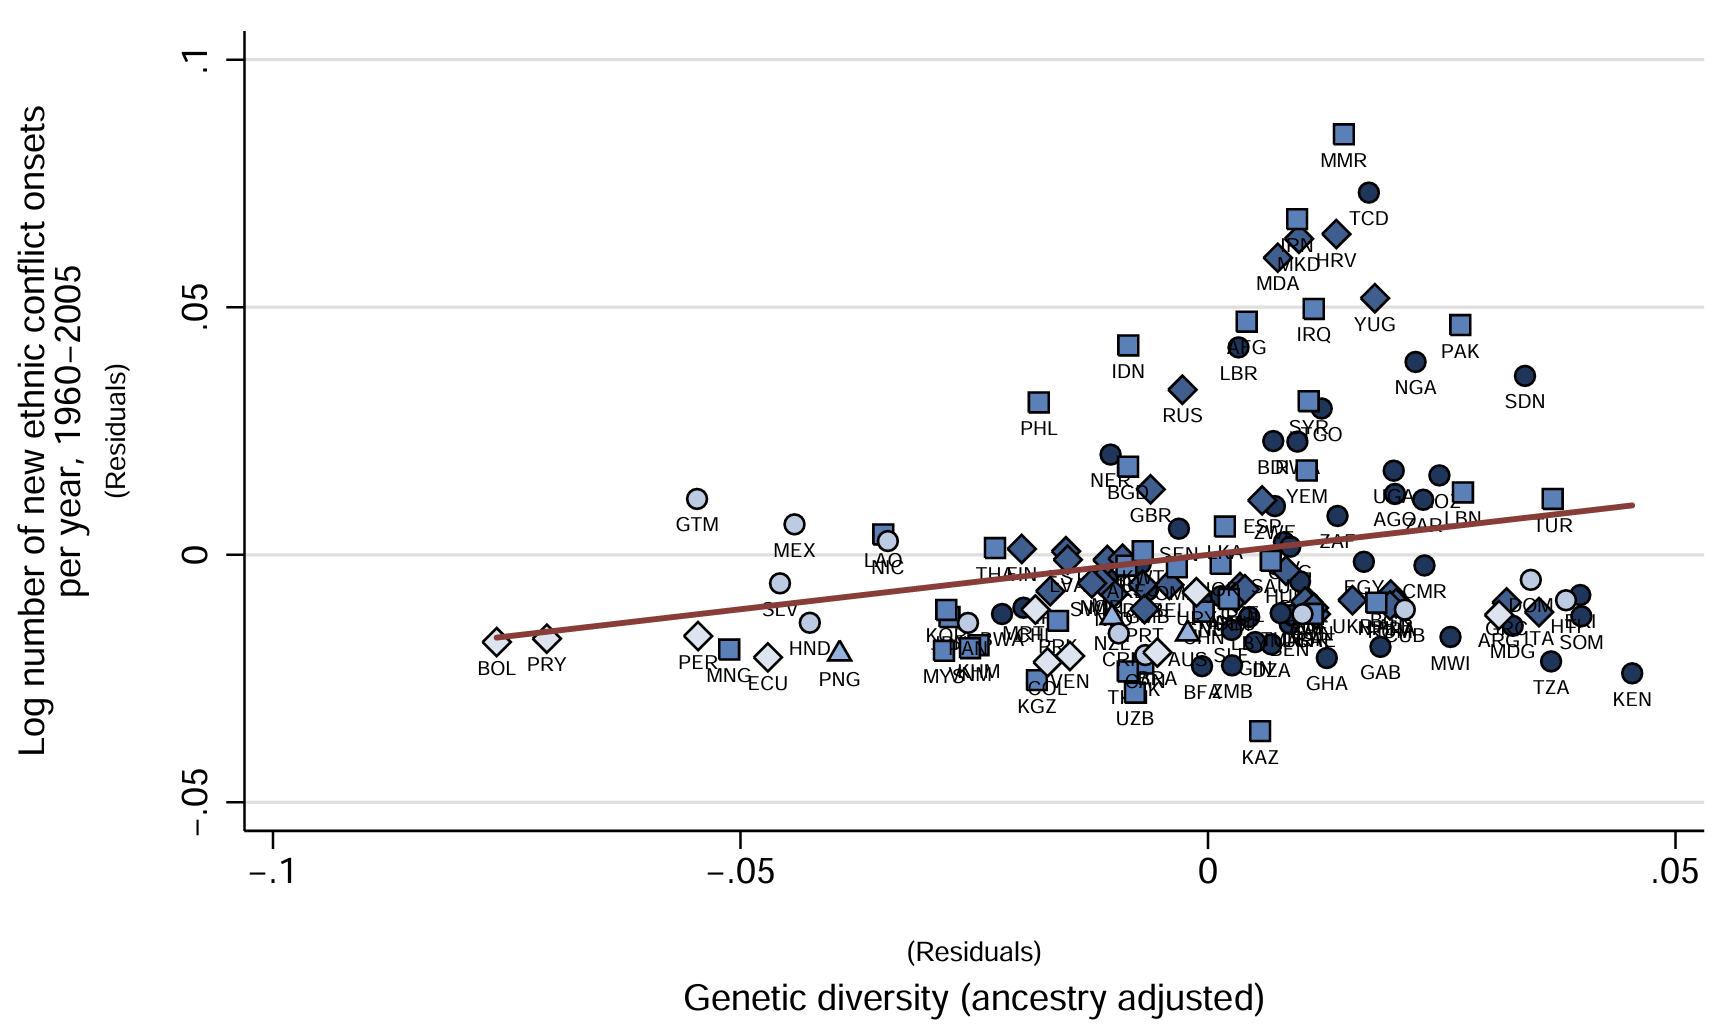
\includegraphics[width=0.75\linewidth]{Linear Regression/Figures/FWL_example.png}
        \caption{The Nature of Conflict (Arbatli, Ashraf, and Galor 2015)}
        \label{fig:placeholder}
    \end{figure}
\end{frame}

\subsection*{Asymptotic Property of OLS}

\begin{frame}
  \subsectionpage
\end{frame}

\begin{frame}{Asymptotic Property of OLS}

We are interested in the distribution of the \textit{sample} analog of 
\begin{align*}
    \beta &= E[X_iX_i']^{-1}E[X_iY_i] \\
    \text{where } X_i &=
    \begin{bmatrix}
    X_{i1} \\
    X_{i2} \\
    \vdots \\
    X_{ip}
    \end{bmatrix}
    \in \mathbb{R}^{p\times 1} \hspace{3pt} 
    \text{and } Y_i \text{ is a } \textit{scalar}
\end{align*}
Suppose $[Y_i X_i']'$ is \textit{independently and identically distributed} in a sample of size $n$. The OLS estimator is given by
\begin{align*}
    \hat{\beta} &= \left[\sum_i X_i X_i' \right]^{-1} \sum_i X_i Y_i
\end{align*}
\end{frame}

\begin{frame}{Asymptotic Property of OLS}
    \begin{itemize}
        \item Given $Y_i = X_i'\beta + e_i$
        \begin{align*}
        \hat{\beta} &= \left[\sum_i X_i X_i' \right]^{-1} \sum_i X_i \left( X_i'\beta + e_i \right) \\
        &= \beta + \left[\sum_i X_i X_i' \right]^{-1} \sum_i X_ie_i
        \end{align*}
        \item Under regularity conditions $E||X_i||^2 < \infty$, $E\left[e_i^2||X_i||^2\right] < \infty$, $E[X_iX_i']$ is  invertible ($E[X_iX_i'] \succ 0$), and $p/n \rightarrow 0$
        \begin{align*}
            \sqrt{n}(\hat{\beta}-\beta) \xrightarrow{d} \mathcal{N}\left( 0, E[X_iX_i']^{-1}E[e_i^2 X_i X_i'] E[X_iX_i']^{-1} \right)
        \end{align*}
    \end{itemize}
\end{frame}

\begin{frame}{Asymptotic Property of OLS}

$\hat \beta$ is $\sqrt{n}$-consistent
\begin{align*}
    \sqrt{n}(\hat{\beta}-\beta) \xrightarrow{d} \mathcal{N}\left( 0, E[X_iX_i']^{-1}E[e_i^2 X_i X_i'] E[X_iX_i']^{-1} \right)
\end{align*}
The consistent ``sandwich'' estimator (Eicker-Huber-White) of a \textit{sample} is then given by
\begin{align*}
    \hat{V}(\hat{\beta}) = (X_iX_i')^{-1}\left( \sum_i^{n} X_iX_i'\hat{e}_i^{2} \right) (X_iX_i')^{-1}
\end{align*}
by plugging in sample $\hat e_i^2$ to estimate $e_i^2$ \\[5pt]

This is also known as heteroskedasticity-consistent standard errors (\textit{robust}).
\end{frame}

\begin{frame}{Asymptotic Property of OLS}

\begin{itemize}
    \item This is, however, not the standard error you get by default from packaged software.
    \item Default standard errors are derived under a homoskedasticity assumption $E[e_i^2|X_i]=\sigma^2$
    \item Given the assumption, we have the ``meat''
    \begin{align*}
        E[e_i^2X_iX_i'] = E[E[e_i^2X_iX_i' | X_i]] = \sigma^2E[X_iX_i']
    \end{align*}
    Accordingly, 
    \begin{align*}
        E[X_iX_i']^{-1}E[e_i^2 X_i X_i'] E[X_iX_i']^{-1} &= \sigma^2 E[X_iX_i']^{-1}E[X_i X_i'] E[X_iX_i']^{-1} \\
        &= \sigma^2E[X_iX_i']^{-1}
    \end{align*}
\end{itemize} 
\end{frame}

\begin{frame}{Asymptotic Property of OLS}

\begin{itemize}
    \item When $p/n$ is not small, the ``sandwich'' estimate becomes inconsistent and underestimated
    \item The last chapter of \textsc{MHE} discusses the issue in detail, and here I give the intuition
    \item when $p/n \rightarrow c > 0$, the \textit{operator norm error} no longer vanishes, but grows at rate of $\sqrt{p/n}$
    $$
    \Big\|\tfrac{1}{n}X_iX_i' - E[X_iX_i']\Big\|_{\mathrm{op}}
    = \sup_{\|v\|_2=1} \left|\,v'\Big(\tfrac{1}{n}X_iX_i' - E[X_iX_i']\Big)v\,\right| \sim \mathcal{O}_p(\sqrt{\frac{p}{n}})
    $$
    \item The intuition is that each entry of $\tfrac{1}{n}X_i'X_i$ still satisfies LLN; however there are $p \times p$ entries. Ensuring all of them to be consistent is much harder, and the LLN fails in operator norm.
\end{itemize}
\end{frame}

\subsection{Neyman Orthogonality}

\begin{frame}
  \subsectionpage
\end{frame}

\begin{frame}{$\beta$ in Multivariate Regression Using a \textit{Sample}}
 \textit{Adaptive Statistical Inference}
 \begin{itemize}
     \item Under regularity conditions and if $p/n \approx 0$, the estimation error in $\check{D}_i$ and $\check{Y}_i$ has no first-order effect on the stochastic behavior of $\hat{\beta}_1$
 \end{itemize}
 \begin{align*}
     \sqrt{n} (\hat \beta_1 - \beta_1) &\xrightarrow{d} \mathcal{N}\left(0, E[\tilde{D}^2]^{-1}E[\tilde{D}^2e^2]E[\tilde{D}^2]^{-1}\right)
 \end{align*}
  \begin{itemize}
     \item Note the sample estimate of $\hat V(\hat \beta_1)$ is the same heteroskedasticity robust standard errors we derived before
 \end{itemize}
\end{frame}

\begin{frame}{Adaptive Statistical Inference}
 \begin{itemize}
     \item The \textit{Adaptive Statistical Inference} points to the fact that estimation of residuals $\check{D}$ has a negligible impact on the large sample behavior of the OLS estimate
     \item The approximate behavior is the same as if we had used true residuals $\check D$ instead
 \end{itemize}
\end{frame}

\begin{frame}{From FWL to Neyman Orthogonality (Quick Summary)}

\begin{itemize}
    \item The \textit{adaptivity} property will be derived later as a consequence of a more general phenomenon called \textit{Neyman orthogonality}
    \item Formally, \[
    \left.\frac{\partial}{\partial \eta} E[\psi(Z;\theta,\eta)]\right|_{\eta=\eta_0} = 0
    \]
    \item where $Z$ is the observed data, $\theta$ is the target parameter, $\eta$ is the estimated nuisance function, and $\eta_0$ is the true nuisance function
    \item $\psi(\cdot)$ is the score function; in the OLS case, it is the normal equation
\end{itemize}
\end{frame}

\begin{frame}{From FWL to Neyman Orthogonality (Quick Summary)}

\textit{Neyman Orthogonality}
\[
    \left.\frac{\partial}{\partial \eta} E[\psi(Z;\theta,\eta)]\right|_{\eta=\eta_0} = 0
    \]
When \textit{Neyman Orthogonality} is satisfied (OLS satisfies it by design)
    \begin{itemize}
        \item Small errors in estimating $\eta$ (that affects moment only at second order) does not change the fact that one still get $\sqrt{n}$-consistent, asymptotically normal inference for $\theta$
        \item One can more flexibly estimate $\eta$, even in the case of non-linearity and high-dimensional data, using machine learning (ML)
        \item This is one of the key motivations of Double Machine Learning (DML)
    \end{itemize}
\end{frame}

\end{document}